\documentclass[12pt,a4paper]{article}
\usepackage[portuguese]{babel}
\usepackage[utf8]{inputenc}
\usepackage[margin=1in]{geometry}
\usepackage{microtype}
\usepackage{amsfonts}
\usepackage{amsthm}
\usepackage{graphicx}

\newcommand{\N}{\mathbb{N}}
\newcommand{\R}{\mathbb{R}}

\theoremstyle{definition}
\newtheorem{ex}{Exercício}[section]

\title{Notas de física básica 1}
\author{Max Jauregui}

\begin{document}
\maketitle
\section{Cinemática em uma dimensão}

\subsection{Sistemas de referência}

Vamos estudar o movimento de um objeto que só pode se mover ao longo
de uma reta. Vamos assumir que as dimensões do objeto não são
importantes para o seu movimento. Assim, vamos considerar que todo
objeto é uma partícula, a qual é representada por um ponto.

Para estudarmos o movimento de uma partícula, é necessário definir
primeiro um \emph{sistema de referência} ou \emph{referencial}, o qual
é constituído por um sistema de coordenadas para determinar posições e
um relógio para medir tempos. No caso particular no qual a partícula
se move ao longo de uma reta, o sistema de coordenadas é composto
simplesmente por um ponto, chamado de \emph{origem} do sistema de
coordenadas, e um eixo, usualmente chamado de \emph{eixo $x$}.

Fixado um referencial, a posição da partícula em um instante $t\ge 0$
é dada por um número real $x(t)$. Isso define uma função
$x:[0,+\infty)\to\R$, a qual, assim como a maioria de funções em
física, assumiremos que tenha derivadas de qualquer ordem.

O sistema internacional de unidades (SI) estabelece o segundo (s) como
a unidade de tempo e o metro (m) como a unidade de comprimento. Nessa
direção, vamos coniderar sempre que $x(t)$ é a posição da partícula
medida em metros no instante $t$, medido em segundos.

\subsection{Velocidade média e velocidade escalar média}

Consideremos uma partícula que se move ao longo de uma linha reta e
suponhamos que conheçamos a posição da partícula em dois instantes
diferentes $t_1$ e $t_2$. A velocidade média da partícula no intervalo
de tempo entre $t_1$ e $t_2$ é definida por
$$\overline v=\frac{x(t_2)-x(t_1)}{t_2-t_1}\,.$$
Introduzindo a notação $\Delta t=t_2-t_1$, podemos escrever
$$\overline{v}=\frac{x(t_1+\Delta t)-x(t_1)}{\Delta t}\,.$$
A unidade de velocidade média no SI é metros por segundo (m/s).

A velocidade média de uma partícula pode ser positiva, negativa ou
nula. Por exemplo, se $x(t_2)=x(t_1)$ (a partícula volta para a mesma
posição), $\overline{v}=0\,\mathrm{m/s}$. Nesse caso, a partícula não
necessariamente ficou parada entre os instantes $t_1$ e $t_2$. De
fato, ela pode ter percorrido uma distância $d\ne 0$ e retornado
finalmente na sua posição de partida. Definimos a \emph{velocidade
  escalar média} da partícula no intervalo de tempo entre $t_1$ e
$t_2$ por
$$v_s=\frac{d}{|\Delta t|}\,,$$
onde $d$ é a distância percorrida pela partícula entre os instantes
$t_1$ e $t_2$.

A velocidade escalar média de uma partícula é sempre não-negativa. A
definição de velocidade escalar média fica inalterada no caso geral do
movimento de uma partícula em três dimensões.

\begin{ex}
  Um cachorro está inicialmente (instante $0\,\mathrm{s}$) na posição
  $0\,\mathrm{m}$. Logo, o cachorro corre para a direita
  $40\,\mathrm{m}$ e depois anda $20\,\mathrm{m}$ para a esquerda,
  chegando na sua posição final no instante $12\,\mathrm{s}$. Encontre
  a velocidade média e a velocidade escalar média do cachorro entre os
  instantes $0\,\mathrm{s}$ e $12\,\mathrm{s}$. \emph{Resposta:}
  $\overline{v}=1{,}7\,\mathrm{m/s}$ e
  $\overline{v}_s=5\,\mathrm{m/s}$.
\end{ex}

\subsection{Velocidade instantânea}

Comecemos com um exemplo.

\begin{ex}
  Uma partícula se move ao longo de uma linha reta e se encontra na
  posição $1{,}0\,\mathrm{m}$ no instante $1{,}0\,\mathrm{s}$. (i) Se
  a partícula está na posição $4{,}0\,\mathrm{m}$ no instante
  $2{,}0\,\mathrm{s}$, encontre a velocidade média da partícula entre
  os instantes $1{,}0\,\mathrm{s}$ e $2{,}0\,\mathrm{s}$. (ii) Suponha
  que a partícula se encontre nas posições $2{,}3\,\mathrm{m}$ e
  $1{,}7\,\mathrm{m}$ nos instantes $1{,}5\,\mathrm{s}$ e
  $1{,}3\,\mathrm{s}$ respectivamente. Determine a velocidade média da
  partícula entre os instantes $1{,}0\,\mathrm{s}$ e
  $1{,}5\,\mathrm{s}$ e entre os instantes $1{,}0\,\mathrm{s}$ e
  $1{,}3\,\mathrm{s}$. \emph{Resposta:} (i) $3{,}0\,\mathrm{m/s}$ (ii)
  $2{,}6\,m\mathrm{m/s}$ e $2{,}3\,\mathrm{m/s}$.
\end{ex}

O exercício anterior ilustra que a velocidade instantânea da partícula
entre os instantes $1{,}0\,\mathrm{s}$ e $t$ se aproxima de
$2\,\mathrm{m/s}$ quando $t$ se aproxima de
$1{,}0\,\mathrm{m/s}$. Isso motiva a dizer que a velocidade da
partícula no instante $1{,}0\,\mathrm{s}$ é $2\,\mathrm{m/s}$. Essa
velocidade é chamada de \emph{velocidade instantânea} e é definida
matematicamente para um instante arbitrário $t$ por
$$v(t)=\lim_{\Delta t\to 0}\frac{x(t+\Delta t)-x(t)}{\Delta t}\,.$$
O limite do lado direito é muito importante e é chamado em cálculo de
derivada da função $x$ no ponto $t$, denotado por $dx/dt$. Logo, temos
que
$$v(t)=\frac{dx}{dt}\,.$$
O valor absoluto da velocidade instantânea é chamado às vezes de
\emph{velocidade escalar instantânea}.

Neste curso essencialmente trabalharemos com funciones
polinomiais. Para calcular a derivada de polinômios, usaremos as
seguintes regras:
\begin{eqnarray*}
  \frac{dt^n}{dt}&=&nt^{n-1}\,,\quad n\in\N\,;\\
  \frac{dc}{dt}&=& 0\,,\quad\mbox{para qualquer constante }c\,.
\end{eqnarray*}

\begin{ex}
  A posição de uma partícula em metros é dada pela expressão
  $x(t)=5t^2-2t+3$ se $t$ é medido em segundos. Encontre a velocidade
  instantânea da partícula no instante
  $2\,\mathrm{s}$. \emph{Resposta:} $18\,\mathrm{m/s}$.
\end{ex}

Tendo os pares $(t,x(t))$ para vários instantes $t$, podemos desenhar
o gráfico da função $x$. Esse gráfico é usualmente chamado de
\emph{gráfico posição versus tempo} ou simplesmente \emph{gráfico $x$
  vs $t$}. A razão $r=[x(t+\Delta t)-x(t)]/\Delta t$ é a inclinação do
segmento que une os pontos $(t,x(t))$ e $(t+\Delta t,x(t+\Delta
t))$. Se $\Delta t$ tende a $0$ ($\Delta t\to 0$), a razão $r$
torna-se a inclinação da reta tangente que passa pelo ponto
$(t,x(t))$. Assim, se temos um gráfico $x$ vs $t$, a velocidade
instantânea em um instante $t$ será dada pela inclinação da reta que é
tangente ao gráfico nesse instante.

\begin{ex}
  Considere o gráfico $x$ vs $t$ dado na Fig.~\ref{fig:xtcurve}. (i)
  Encontre os valores aproximados dos instantes onde a velocidade
  instantânea é $0\,\mathrm{m/s}$. (ii) Encontre o valor aproximado do
  instante em que a partícula se move de direita a esquerda com
  velocidade escalar instantânea máxima.
  \begin{figure}[ht]
    \centering
    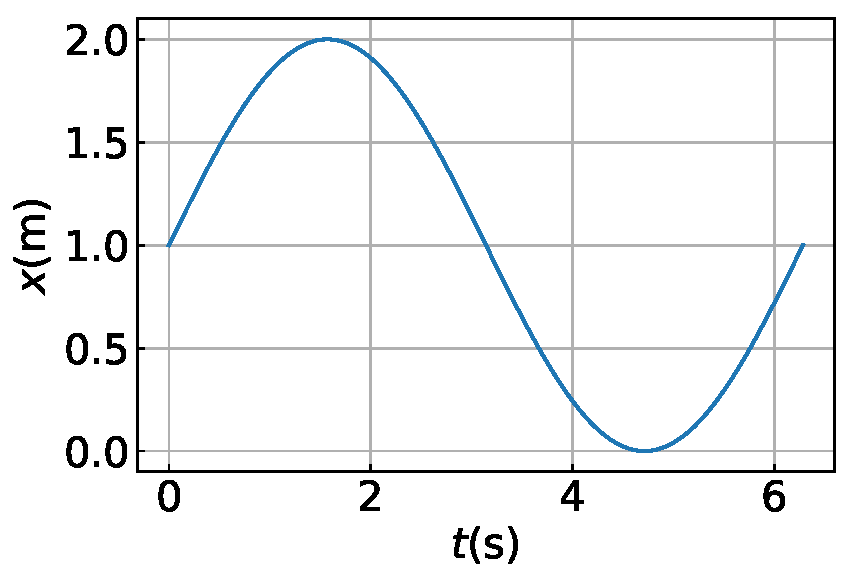
\includegraphics[width=0.5\textwidth,keepaspectratio]{xtcurve.pdf}
    \caption{$x$ vs $t$ graph.}
    \label{fig:xtcurve}
  \end{figure}
\end{ex}

\end{document}